\section{Motivation and Scope}

There has been a strong desire for a more space- and/or runtime-efficient
representation for \code{map} among C++ users for some time now.  This has
motivated discussions among the members of SG14, numerous articles and talks,
and an implementation in Boost, \code{boost::container::flat_map}.  Virtually
everyone who makes games, embedded, or system software in C++ uses the Boost
implementation or one that they rolled themselves.\\

Here are some numbers that show why.  The graphs that follow show runtimes for
different \code{map}-like associative containers.  The containers used are
Boost.FlatMap, \code{std::map}, and two thin wrappers over a sorted
\code{std::vector}; the ``custom pair'' version of the sorted
\code{std::vector} uses a simple \code{struct} instead of \code{std::pair} for
its value type.  All containers use an \code{int} as the key type and an
\code{int} or a \code{struct} with 5 \code{double}s for the value type.\\

These first three graphs cover the \code{int}-value-type case.  The first
graph shows insertion of N elements with random keys; the second shows full
iteration across all N elements; and the third shows erasure of all N
elements, by the keys used in the original insertions.

\begin{center}
    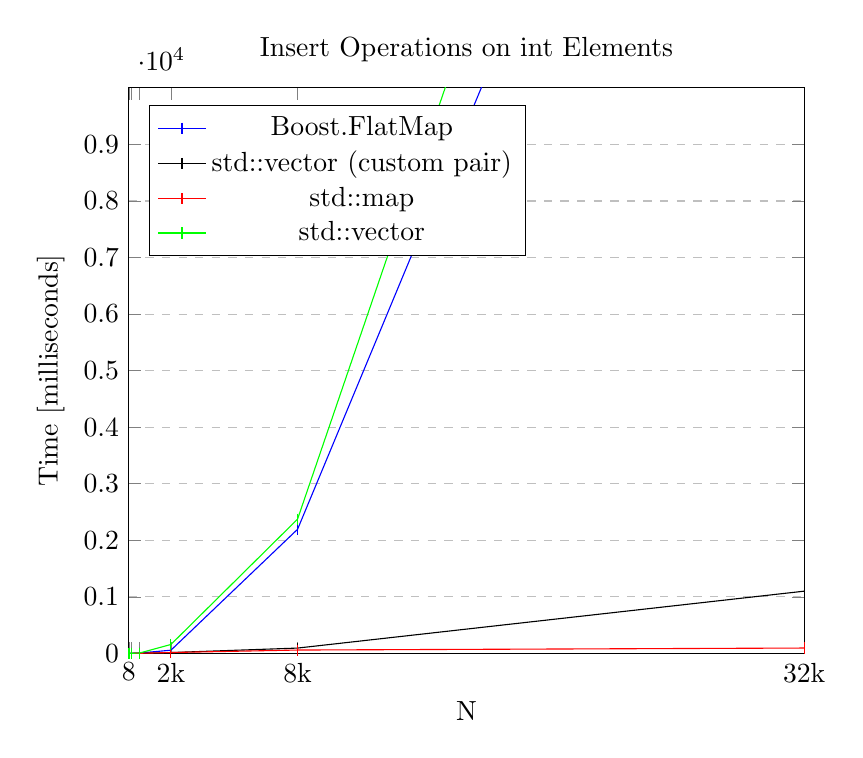
\begin{tikzpicture}
    \begin{axis}[
        width=4in,
        title={Insert Operations on int Elements},
        xlabel={N},
        ylabel={Time [milliseconds]},
        xmin=0, xmax=32768.0,
        ymin=0, ymax=10000.0,
        xtick={8,32,128,512,2048,8192,32768},
        xticklabels={8,,,,2k,8k,32k},
        ytick={0.0,1000.0,2000.0,3000.0,4000.0,5000.0,6000.0,7000.0,8000.0,9000.0},
        legend pos=north west,
        ymajorgrids=true,
        grid style=dashed,
        scaled x ticks=false,
        legend entries={Boost.FlatMap,std::vector (custom pair),std::map,std::vector},
        ]

    \addplot[color=blue,mark=|,]
        coordinates {(8,0.069911)(32,0.302622)(128,1.42784)(512,5.56055)(2048,55.7729)(8192,2194.15)(32768,23721.7)};

    \addplot[color=black,mark=|,]
        coordinates {(8,0.034153)(32,0.169993)(128,0.606432)(512,1.32712)(2048,14.2242)(8192,93.3417)(32768,1099.65)};

    \addplot[color=red,mark=|,]
        coordinates {(8,0.040857)(32,0.199188)(128,0.730959)(512,1.12619)(2048,14.5855)(8192,58.5812)(32768,94.0076)};

    \addplot[color=green,mark=|,]
        coordinates {(8,0.024585)(32,0.214133)(128,1.18521)(512,4.36878)(2048,156.937)(8192,2374.02)(32768,28552.8)};

    \end{axis}
\end{tikzpicture}
\end{center}

\begin{center}
    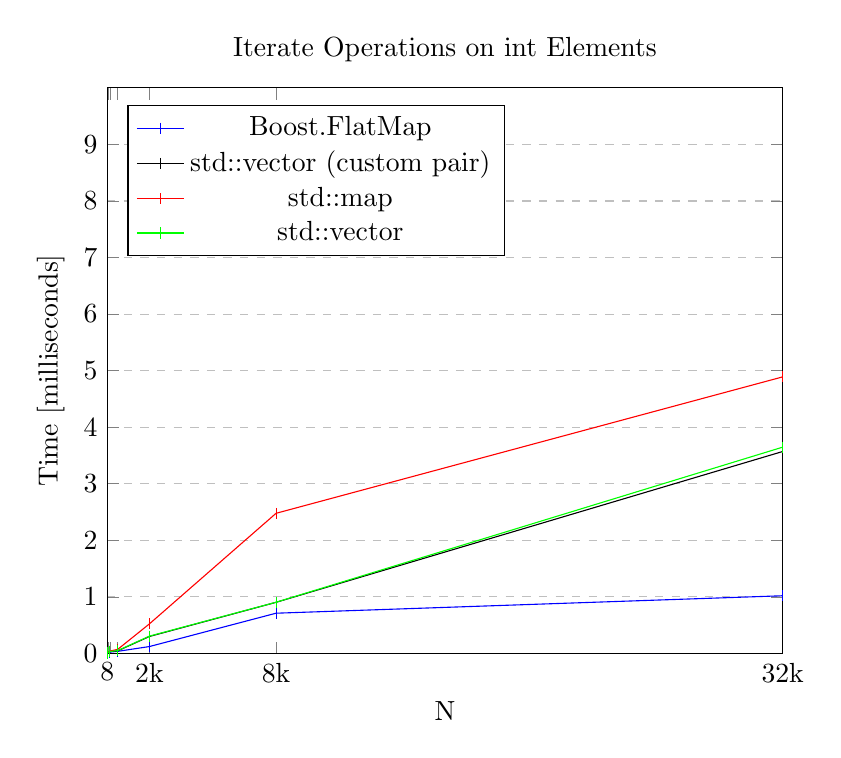
\begin{tikzpicture}
    \begin{axis}[
        width=4in,
        title={Iterate Operations on int Elements},
        xlabel={N},
        ylabel={Time [milliseconds]},
        xmin=0, xmax=32768.0,
        ymin=0, ymax=10.0,
        xtick={8,32,128,512,2048,8192,32768},
        xticklabels={8,,,,2k,8k,32k},
        ytick={0.0,1.0,2.0,3.0,4.0,5.0,6.0,7.0,8.0,9.0},
        legend pos=north west,
        ymajorgrids=true,
        grid style=dashed,
        scaled x ticks=false,
        legend entries={Boost.FlatMap,std::vector (custom pair),std::map,std::vector},
        ]

    \addplot[color=blue,mark=|,]
        coordinates {(8,0.001607)(32,0.014177)(128,0.021511)(512,0.03548)(2048,0.120266)(8192,0.709866)(32768,1.0185)};

    \addplot[color=black,mark=|,]
        coordinates {(8,0.001746)(32,0.015365)(128,0.033454)(512,0.044489)(2048,0.298292)(8192,0.902349)(32768,3.56938)};

    \addplot[color=red,mark=|,]
        coordinates {(8,0.002933)(32,0.017111)(128,0.039111)(512,0.071028)(2048,0.520877)(8192,2.47664)(32768,4.88896)};

    \addplot[color=green,mark=|,]
        coordinates {(8,0.001746)(32,0.015365)(128,0.032407)(512,0.049238)(2048,0.304647)(8192,0.903956)(32768,3.64641)};

    \end{axis}
\end{tikzpicture}
\end{center}

\begin{center}
    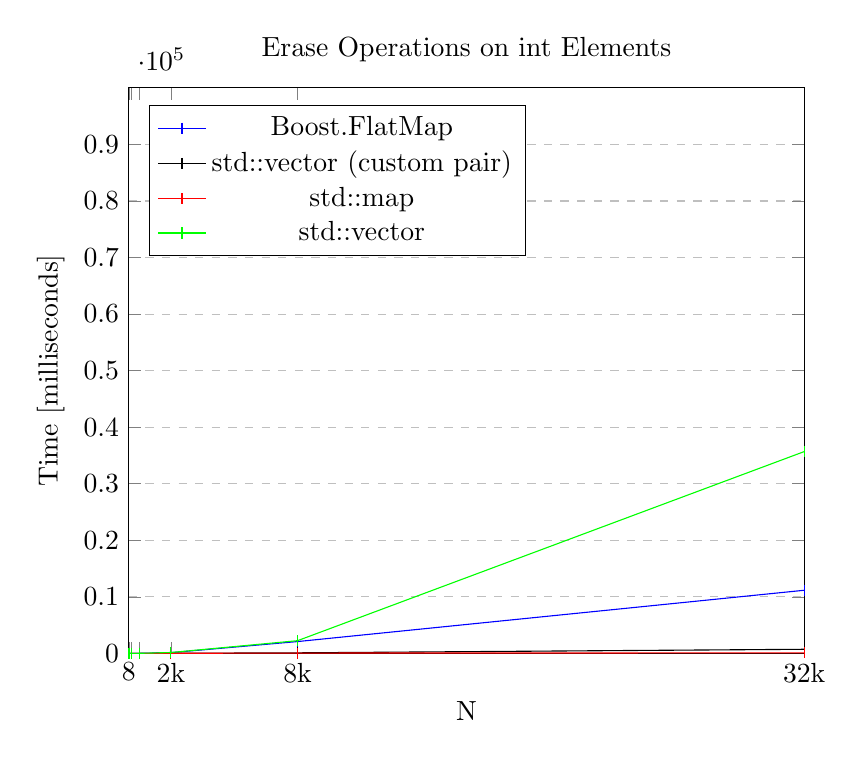
\begin{tikzpicture}
    \begin{axis}[
        width=4in,
        title={Erase Operations on int Elements},
        xlabel={N},
        ylabel={Time [milliseconds]},
        xmin=0, xmax=32768.0,
        ymin=0, ymax=100000.0,
        xtick={8,32,128,512,2048,8192,32768},
        xticklabels={8,,,,2k,8k,32k},
        ytick={0.0,10000.0,20000.0,30000.0,40000.0,50000.0,60000.0,70000.0,80000.0,90000.0},
        legend pos=north west,
        ymajorgrids=true,
        grid style=dashed,
        scaled x ticks=false,
        legend entries={Boost.FlatMap,std::vector (custom pair),std::map,std::vector},
        ]

    \addplot[color=blue,mark=|,]
        coordinates {(8,0.022349)(32,0.198419)(128,1.06271)(512,3.71137)(2048,122.628)(8192,2083.85)(32768,11155.7)};

    \addplot[color=black,mark=|,]
        coordinates {(8,0.017531)(32,0.138565)(128,0.55901)(512,1.30366)(2048,14.1557)(8192,90.8456)(32768,719.457)};

    \addplot[color=red,mark=|,]
        coordinates {(8,0.019834)(32,0.156165)(128,0.568019)(512,0.928749)(2048,11.4119)(8192,49.8328)(32768,81.8665)};

    \addplot[color=green,mark=|,]
        coordinates {(8,0.021441)(32,0.181517)(128,1.08638)(512,4.14138)(2048,150.503)(8192,2241.38)(32768,35677.9)};

    \end{axis}
\end{tikzpicture}
\end{center}


These next three graphs are just like the preceding ones, but cover the
\code{struct}-value-type case.

\begin{center}
    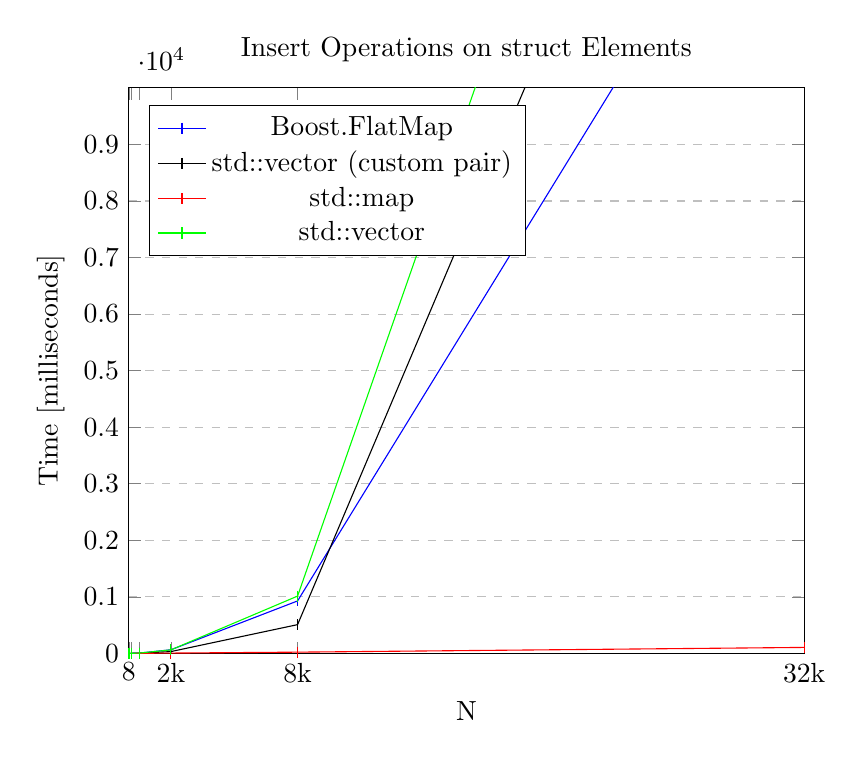
\begin{tikzpicture}
    \begin{axis}[
        width=4in,
        title={Insert Operations on struct Elements},
        xlabel={N},
        ylabel={Time [milliseconds]},
        xmin=0, xmax=32768.0,
        ymin=0, ymax=10000.0,
        xtick={8,32,128,512,2048,8192,32768},
        xticklabels={8,,,,2k,8k,32k},
        ytick={0.0,1000.0,2000.0,3000.0,4000.0,5000.0,6000.0,7000.0,8000.0,9000.0},
        legend pos=north west,
        ymajorgrids=true,
        grid style=dashed,
        scaled x ticks=false,
        legend entries={Boost.FlatMap,std::vector (custom pair),std::map,std::vector},
        ]

    \addplot[color=blue,mark=|,]
        coordinates {(8,0.036737)(32,0.100921)(128,0.549651)(512,5.00853)(2048,63.213)(8192,926.91)(32768,15505.9)};

    \addplot[color=black,mark=|,]
        coordinates {(8,0.024585)(32,0.066488)(128,0.337194)(512,2.68142)(2048,31.3329)(8192,507.779)(32768,21672.2)};

    \addplot[color=red,mark=|,]
        coordinates {(8,0.025841)(32,0.070819)(128,0.265047)(512,1.02932)(2048,4.63257)(8192,21.1444)(32768,104.896)};

    \addplot[color=green,mark=|,]
        coordinates {(8,0.025423)(32,0.084438)(128,0.475061)(512,4.77959)(2048,61.6609)(8192,1012.57)(32768,26664.8)};

    \end{axis}
\end{tikzpicture}
\end{center}

\begin{center}
    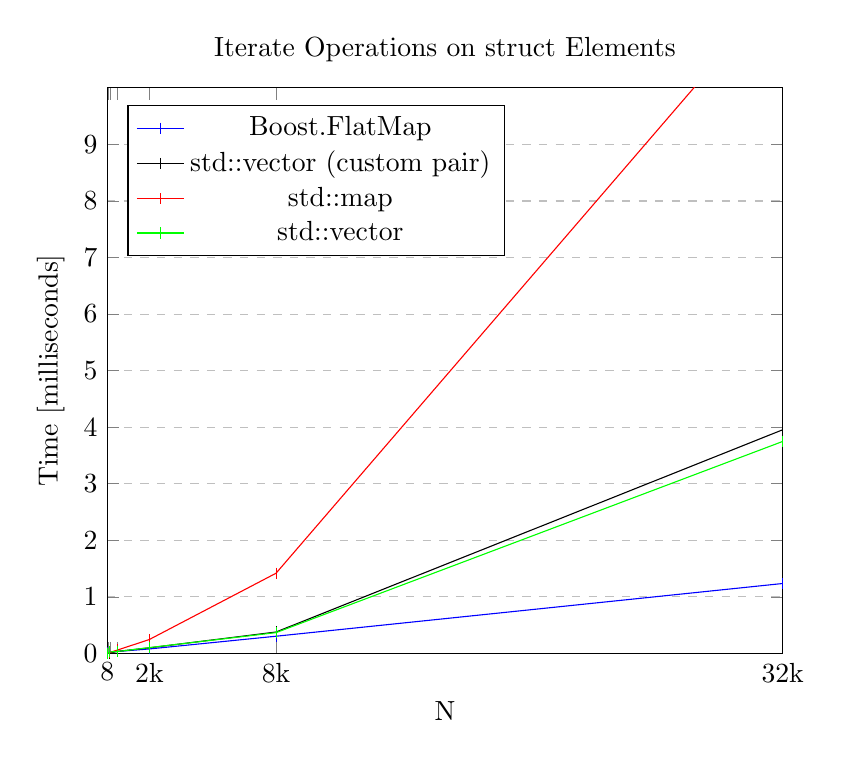
\begin{tikzpicture}
    \begin{axis}[
        width=4in,
        title={Iterate Operations on struct Elements},
        xlabel={N},
        ylabel={Time [milliseconds]},
        xmin=0, xmax=32768.0,
        ymin=0, ymax=10.0,
        xtick={8,32,128,512,2048,8192,32768},
        xticklabels={8,,,,2k,8k,32k},
        ytick={0.0,1.0,2.0,3.0,4.0,5.0,6.0,7.0,8.0,9.0},
        legend pos=north west,
        ymajorgrids=true,
        grid style=dashed,
        scaled x ticks=false,
        legend entries={Boost.FlatMap,std::vector (custom pair),std::map,std::vector},
        ]

    \addplot[color=blue,mark=|,]
        coordinates {(8,0.00887)(32,0.002375)(128,0.024235)(512,0.033454)(2048,0.078013)(8192,0.302902)(32768,1.23514)};

    \addplot[color=black,mark=|,]
        coordinates {(8,0.001187)(32,0.002234)(128,0.006635)(512,0.03534)(2048,0.098266)(8192,0.377352)(32768,3.95344)};

    \addplot[color=red,mark=|,]
        coordinates {(8,0.001467)(32,0.002863)(128,0.016273)(512,0.059645)(2048,0.245353)(8192,1.41708)(32768,11.825)};

    \addplot[color=green,mark=|,]
        coordinates {(8,0.001187)(32,0.002444)(128,0.024933)(512,0.032826)(2048,0.101479)(8192,0.366387)(32768,3.74713)};

    \end{axis}
\end{tikzpicture}
\end{center}

\begin{center}
    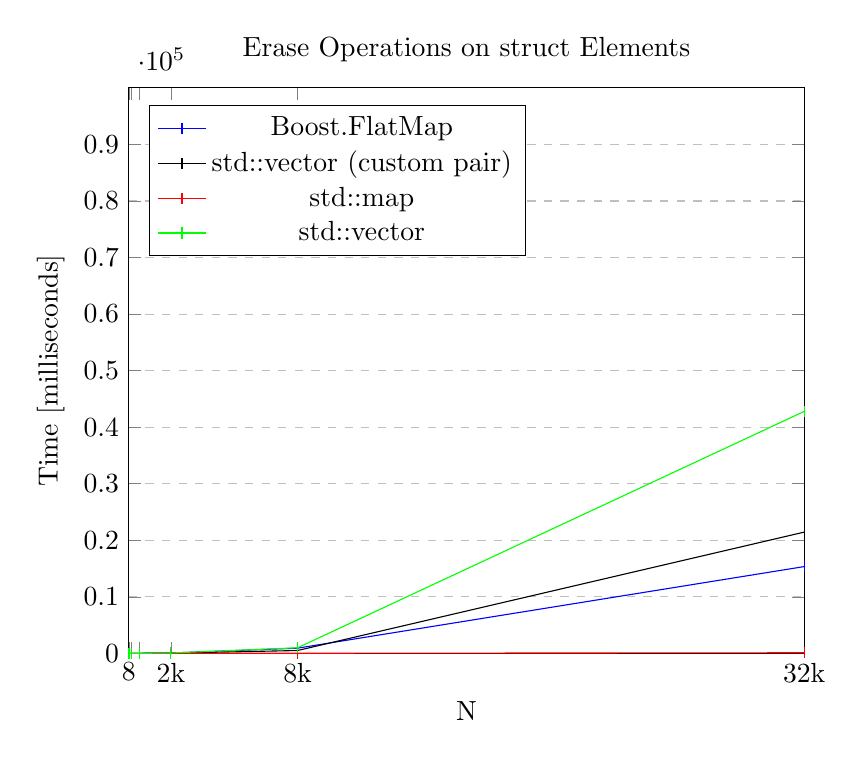
\begin{tikzpicture}
    \begin{axis}[
        width=4in,
        title={Erase Operations on struct Elements},
        xlabel={N},
        ylabel={Time [milliseconds]},
        xmin=0, xmax=32768.0,
        ymin=0, ymax=100000.0,
        xtick={8,32,128,512,2048,8192,32768},
        xticklabels={8,,,,2k,8k,32k},
        ytick={0.0,10000.0,20000.0,30000.0,40000.0,50000.0,60000.0,70000.0,80000.0,90000.0},
        legend pos=north west,
        ymajorgrids=true,
        grid style=dashed,
        scaled x ticks=false,
        legend entries={Boost.FlatMap,std::vector (custom pair),std::map,std::vector},
        ]

    \addplot[color=blue,mark=|,]
        coordinates {(8,0.018298)(32,0.053778)(128,0.417581)(512,4.1066)(2048,60.6217)(8192,918.988)(32768,15343.2)};

    \addplot[color=black,mark=|,]
        coordinates {(8,0.016971)(32,0.051892)(128,0.304927)(512,2.45792)(2048,32.2945)(8192,501.866)(32768,21440)};

    \addplot[color=red,mark=|,]
        coordinates {(8,0.016902)(32,0.047701)(128,0.193112)(512,0.842076)(2048,3.71674)(8192,17.5163)(32768,102.89)};

    \addplot[color=green,mark=|,]
        coordinates {(8,0.016902)(32,0.06593)(128,0.41346)(512,4.11924)(2048,60.78)(8192,984.497)(32768,42785.3)};

    \end{axis}
\end{tikzpicture}
\end{center}


TODO
